The analysis of the results produced by our code passed through a series of intermediate and progressive steps, continuously checking the outcomes obtained via the simulation with the analytical formulas, fortunately available for the non-interacting case. We will now proceed with the presentation of the results derived within the context of our project, enlightening the features of any performed simulation and the methods to validate the solidity and efficiency of the code. First we will focus on the runs carried out in non-interacting case both with the brute-force Metropolis algorithm and the importance sampling, proceeding then towards a more detailed statistical analysis through the blocking method. Then the interaction between particles will be introduced, together with the gradient descent method for the research of the $\alpha$ which minimizes the energy and then concluding with the one-body density evaluation.


\subsection{NON-INTERACTING SYMMETRICAL CASE}
\subsubsection{BRUTE-FORCE METROPOLIS ALGORITHM}
At first we chose a spherical potential trap with a simple gaussian trial wavefunction, these obtained by setting $a=0$ and $\beta=1$ into Eq.\,\ref{wavefunctions} and adopting the potential described in Eq.\,\ref{spherical_pot}. In order to obtain a numerical estimation of the ground state energy of the system we first adopted the so called Brute-Force Metropolis algorithm, previously introduced. We performed different simulations varying many parameters of the system and before each of these runs the system was submitted to $10^5$ thermalization steps. This choice has been preserved for each simulation presented from now on in the report. In principle we could have reduced the number of thermalization steps for the most simple configurations, involving for example 1 particle in a 1-dimensional system. However, since the most time-demanding operation is the evaluation of the local energy (not performed for the thermalization steps), the computational time for the initialization is considerably low, even with such an amount of steps and a large number of particles. We notice also that with the highest number of particles adopted for the system ($N=500$), within a $10^5$-steps thermalization process each of them will on average be moved 200 times, which we retained sufficient for the considered Markov chain to converge to the stationary PDF. \\

Table \ref{tab:tab_x_metropolis_analytical} reports the results of the analysis of the system's dependence on the number of particles and dimension. The value of $\alpha$ was kept fixed at $\alpha = 0.5$. The corresponding results obtained using the numerical method to evaluate the second derivative are reported in Table \ref{tab:tab_x_metropolis_numerical}. One can immediately notice a reduction in the precision and a significant increase in the simulation time with the numerical approach, hence leaving the only purpose of this second method to perform preliminary tests and qualitative studies. Proceeding, Figure \ref{fig:varying_alpha_noninteract_metropolis}, shows the value of the ground state energy of the system as a function of the parameter $\alpha$ for a particular configuration of the simulation settings, that is $N=10$ particles, 3 dimensions, $2^{21}$ steps and Metropolis step-size $r_{step} = 1.0$. One can immediately notice that the function is convex, which guarantees the existence of one unique minimum point, in accordance to what discussed in the context of the gradient descent method. In this simple case, the convexity of the energy curve as a function of $\alpha$ was expected, as it can be derived from the analytical form available in Eq.\,\ref{energy_analitical}. Some selected results for different $\alpha$ values are reported also in Table \ref{tab:varying_alpha_noninteracting}, referring to simulations performed again for a $3D$ system with $N=10$ particles and $N_{steps}=2^{21}$. This table contains also a comparison between the variance calculated as $\sigma^2_E = (\langle E_L^2 \rangle - \langle E_L \rangle^2)/N_{steps}$ and the variance calculated via the blocking method as explained in Section \ref{sec:blocking_method}.

\begin{table}[H]
    \centering
    \begin{tabular}{cccccc}
    \toprule
    $N_{part}$ & $N_{dim}$ & $\langle E_L \rangle$ & $\sigma_E$ & $t_{CPU}\;[s]$ & acc.ratio \\
    \midrule
    1 & 1 & 0.50000 & 0.00000 & 0.250 & 0.7293 \\
    1 & 2 & 1.0000 & 0.00000 & 0.277 & 0.5958 \\
    1 & 3 & 1.5000 & 0.00000 & 0.293 & 0.5053 \\
    \midrule
    10 & 1 & 5.0000 & 0.00000 & 0.397 & 0.7290 \\
    10 & 2 & 10.000 & 0.00000 & 0.426 & 0.5956 \\
    10 & 3 & 15.000 & 0.00000 & 0.453 & 0.5047 \\
    \midrule
    100 & 1 & 50.000 & 0.00000 & 1.967 & 0.7287 \\
    100 & 2 & 100.00 & 0.00000 & 2.084 & 0.5950 \\
    100 & 3 & 150.00 & 0.00000 & 2.388 & 0.5043 \\
    \midrule
    500 & 1 & 250.00 & 0.00000 & 20.695 & 0.7293 \\
    500 & 2 & 500.00 & 0.00000 & 22.008 & 0.5961 \\
    500 & 3 & 750.00 & 0.00000 & 21.776 & 0.5051 \\
    \bottomrule
    \end{tabular}
    \caption{The table reports the results of the simulations performed in the non-interacting case using a simple gaussian trial wavefunction and a brute-force Metropolis sampling method with $N_{therm}=10^5$, $N_{steps}=2^{21}$, step-size set to $r_{step}=1.0$ and constant value for $\alpha=0.5$. The local energy is evaluated exploiting the analytical formula and $\sigma_E$ is the error on $\langle E_L \rangle$ estimated from the standard deviation of of the $E_L$ samples generated during the run. }
    \label{tab:tab_x_metropolis_analytical}
\end{table}

\begin{table}[H]
    \centering
    \begin{tabular}{cccccc}
    \toprule
    $N_{part}$ & $N_{dim}$ & $\langle E_L \rangle $ & $\sigma_E$ & $t_{CPU}$ & acc.ratio \\
    \midrule
    1 & 1 & 0.5000000000 & 7\e-10 & 0.497 & 0.7290 \\
    1 & 2 & 1.000000000 & 1\e-9 & 0.631 & 0.5949 \\
    1 & 3 & 1.500000000 & 2\e-9 & 0.799 & 0.5050 \\
    \midrule
    10 & 1 & 5.000000006 & 2\e-9 & 2.217 & 0.7296 \\
    10 & 2 & 10.000000000 & 3\e-9 & 2.975 & 0.5960 \\
    10 & 3 & 15.000000010 & 5\e-9 & 4.035 & 0.5051 \\
    \midrule
    100 & 1 & 49.999999913 & 7\e-9 & 20.71 & 0.7287 \\
    100 & 2 & 99.99999991 & 1\e-8 & 28.49 & 0.5957\\
    100 & 3 & 149.99999965 & 2\e-8 & 37.02 & 0.5057 \\
    \midrule
    500 & 1 & 250.99999950 & 1\e-8 & 237.05 & 0.7298 \\
    500 & 2 & 500.00000067 & 2\e-8 & 347.24 & 0.5952 \\
    500 & 3 & 749.99999921 & 3\e-8 & 413.98 & 0.5045 \\
    \bottomrule
    \end{tabular}
    \caption{The table reports the results of the simulations in the non-interacting case using a simple gaussian trial wavefunction and a brute-force Metropolis sampling method with $N_{therm}=10^5$,  $N_{steps}=2^{21}$, step-size set to $r_{step}=1.0$ and constant value for $\alpha=0.5$. The local energy is evaluated exploiting the numerical second derivative and $\sigma_E$ is the error on $\langle E_L \rangle$ estimated from the standard deviation of the $E_L$ samples generated during the run. }
    \label{tab:tab_x_metropolis_numerical}
\end{table}

\begin{figure}[H]
    \centering
    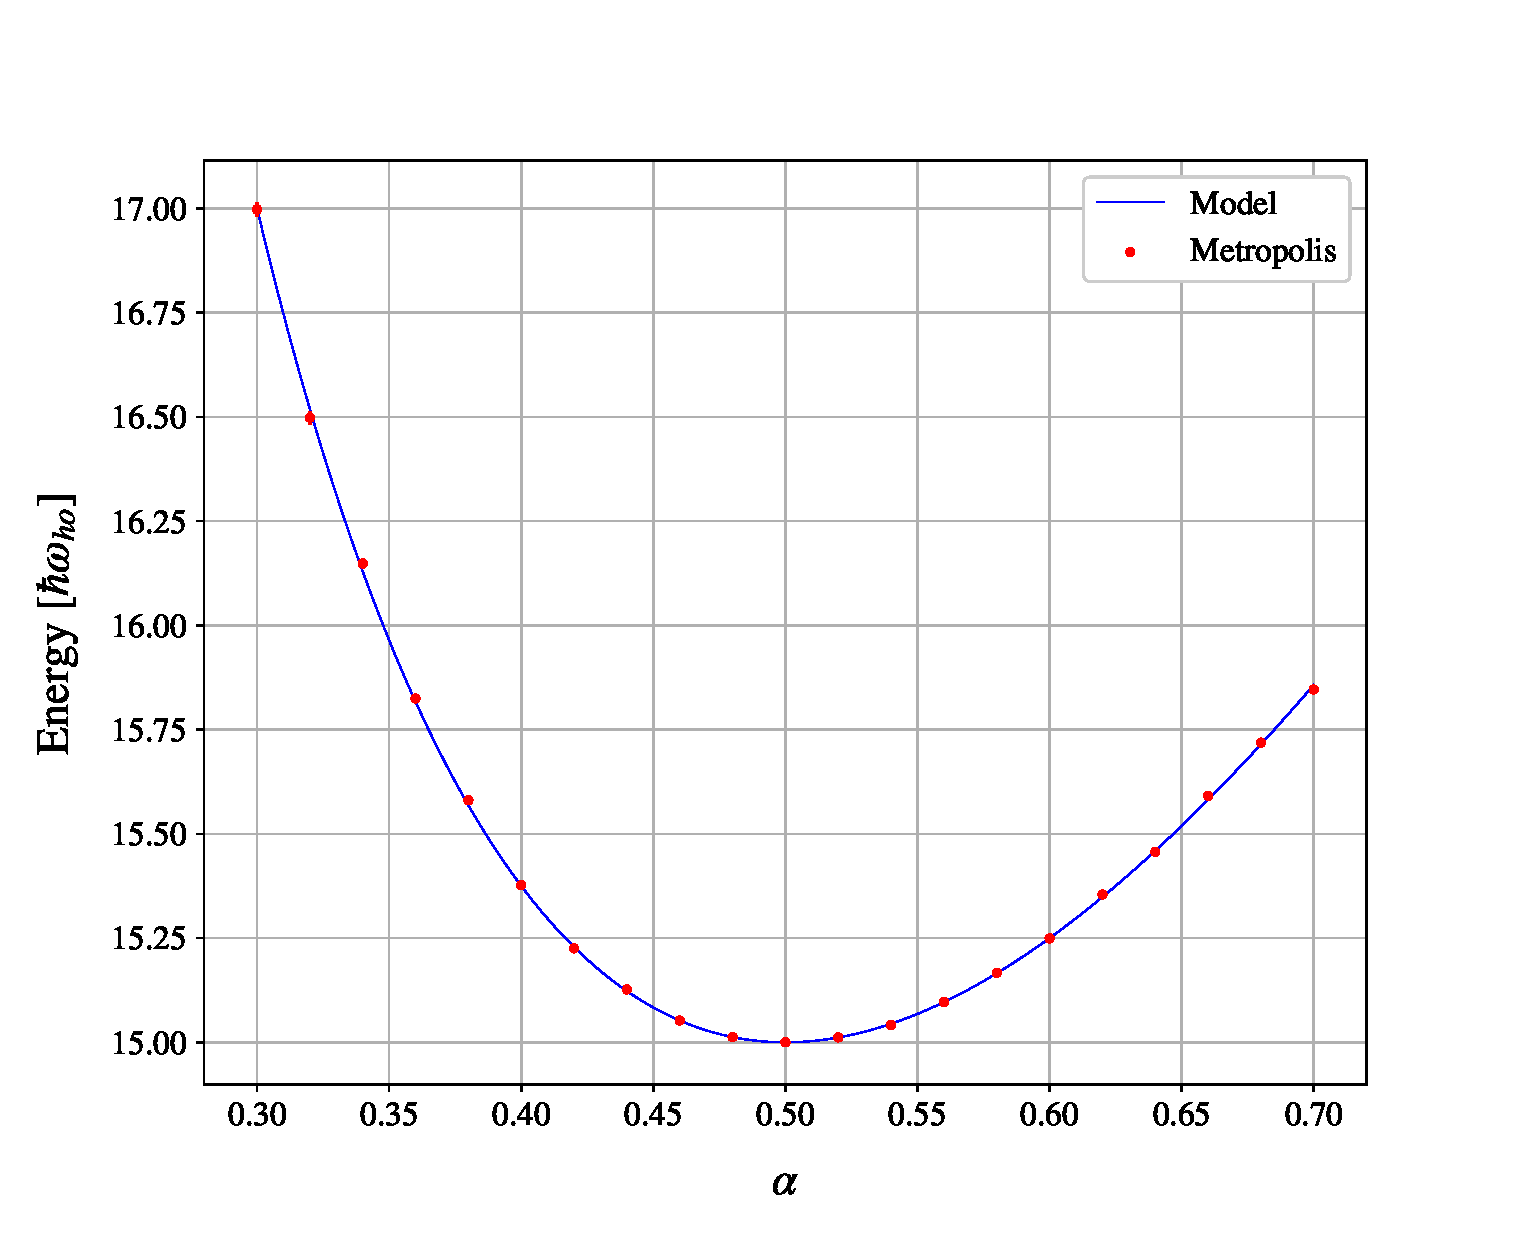
\includegraphics[scale=0.37]{images/varying_alpha_noninteract_metropolis.eps}
    \caption{The figure reports the energy estimates as a function of $\alpha$ generated by various VMC simulations exploiting the brute-force Metropolis algorithm with $N_{therm}=10^5$, $N_{steps}=2^{21}$ and $r_{step}=1.0$. The curve is referred to a $3D$ system with $N=10$ non-interacting particles. For some of the points the errorbar is too small to be seen. }
    \label{fig:varying_alpha_noninteract_metropolis}
\end{figure}


\subsubsection{IMPORTANCE SAMPLING}
The immediate improvement of this simple model was the inclusion of the importance sampling. This allowed us to bias the random walk in the configuration space according to the probability distribution, leading thus to higher number of accepted steps in the Monte Carlo run. As for the Brute Force Metropolis, results for fixed $\alpha=0.5$ obtained with the analytical and numerical evaluation of the local energy are reported respectively in Table \ref{tab:tab_x_importance_analytical} and Table \ref{tab:tab_x_importance_numerical}. The estimated energy as a function of $\alpha$ for a $3D$ system populated by 10 particles is reported in Figure \ref{fig:varying_alpha_noninteract_importance} with some selected results in Table \ref{tab:varying_alpha_noninteracting}. All the simulations cited above have been carried out with $2^{21}$ Monte Carlo steps and $\delta t = 0.1$. 


\begin{table}[H]
    \centering
    \begin{tabular}{cccccc}
    \toprule
    $N_{part}$ & $N_{dim}$ & $\langle E_L \rangle$ & $\sigma_E$ & $t_{CPU}$ & acc. ratio \\
    \midrule
    1 & 1 & 0.50000 & 0.00000 & 0.373 & 0.9928  \\
    1 & 2 & 1.0000 & 0.00000 & 0.385 & 0.98877 \\
    1 & 3 & 1.5000 & 0.00000 & 0.432 & 0.9857 \\
    \midrule
    10 & 1 & 5.0000 & 0.00000 & 0.714 & 0.9929 \\
    10 & 2 & 10.000 & 0.00000 & 0.792 & 0.9889 \\
    10 & 3 & 15.000 & 0.00000 & 0.793 &  0.9858 \\
    \midrule
    100 & 1 & 50.000 & 0.00000 & 4.197 & 0.9929 \\
    100 & 2 & 100.00 & 0.00000 & 4.378 & 0.9887 \\
    100 & 3 & 150.00 & 0.00000 &  4.339 & 0.9856 \\
    \midrule
    500 & 1 & 250.00 & 0.00000 & 36.624 & 0.9929 \\
    500 & 2 & 500.00 & 0.00000 & 39.380 & 0.9888 \\
    500 & 3 & 750.00 & 0.00000 & 39.965 & 0.9858 \\
    \bottomrule
    \end{tabular}
    \caption{The table reports the results of the simulations in the non-interacting case using a simple gaussian trial wavefunction and the importance sampling method with $N_{therm}=10^5$, $N_{steps}=2^{21}$, $\delta t = 0.1$ and constant value for $\alpha=0.5$. The local energy is evaluated exploiting the analytical formula and $\sigma_E$ is the error on $\langle E_L \rangle$ estimated from the standard deviation of the $E_L$ samples generated during the run. }
    \label{tab:tab_x_importance_analytical}
\end{table}

\begin{table}[H]
    \centering
    \begin{tabular}{cccccc}
    \toprule
    $N_{part}$ & $N_{dim}$ & $\langle E_L \rangle$ & $\sigma_E$ & $t_{CPU}$ & acc.ratio \\
    \midrule
    1 & 1 & 0.5000000027 & 7\e-10 & 0.761 & 0.9928 \\
    1 & 2 & 1.000000000 & 1\e-9 & 0.961 & 0.9888 \\
    1 & 3 & 1.500000004 & 2\e-9 &  1.332 & 0.9856\\
    \midrule
    10 & 1 & 4.999999937 & 2\e-9 & 3.311 & 0.9928 \\
    10 & 2 & 10.000000039 & 3\e-9 & 5.772 & 0.9887 \\
    10 & 3 & 15.000000053 & 5\e-9 & 8.097 & 0.9857 \\
    \midrule
    100 & 1 & 49.999999990 & 7\e-9 & 31.444 & 0.9929 \\
    100 & 2 & 99.99999966 & 1\e-8 & 55.850 & 0.9888 \\
    100 & 3 & 150.00000048 & 2\e-8 & 85.201 & 0.9857 \\
    \midrule
    500 & 1 & 250.00000078 & 1\e-8 & 323.70 & 0.9927 \\
    500 & 2 & 500.00000208 & 2\e-8 & 540.58 & 0.9886 \\
    500 & 3 & 749.99999858 & 3\e-8 & 877.82 & 0.9859 \\
    \bottomrule
    \end{tabular}
    \caption{The table reports the results of the simulations in the non-interacting case using a simple gaussian trial wavefunction and the importance sampling method with $N_{therm}=10^5$, $N_{steps}=2^{21}$, $\delta t = 0.1$ and constant value for $\alpha=0.5$. The local energy is evaluated exploiting the numerical evaluation of the second derivative and $\sigma_E$ is the error on $\langle E_L \rangle$ estimated from the standard deviation of the $E_L$ samples generated during the run.  }
    \label{tab:tab_x_importance_numerical}
\end{table}

\begin{figure}[H]
    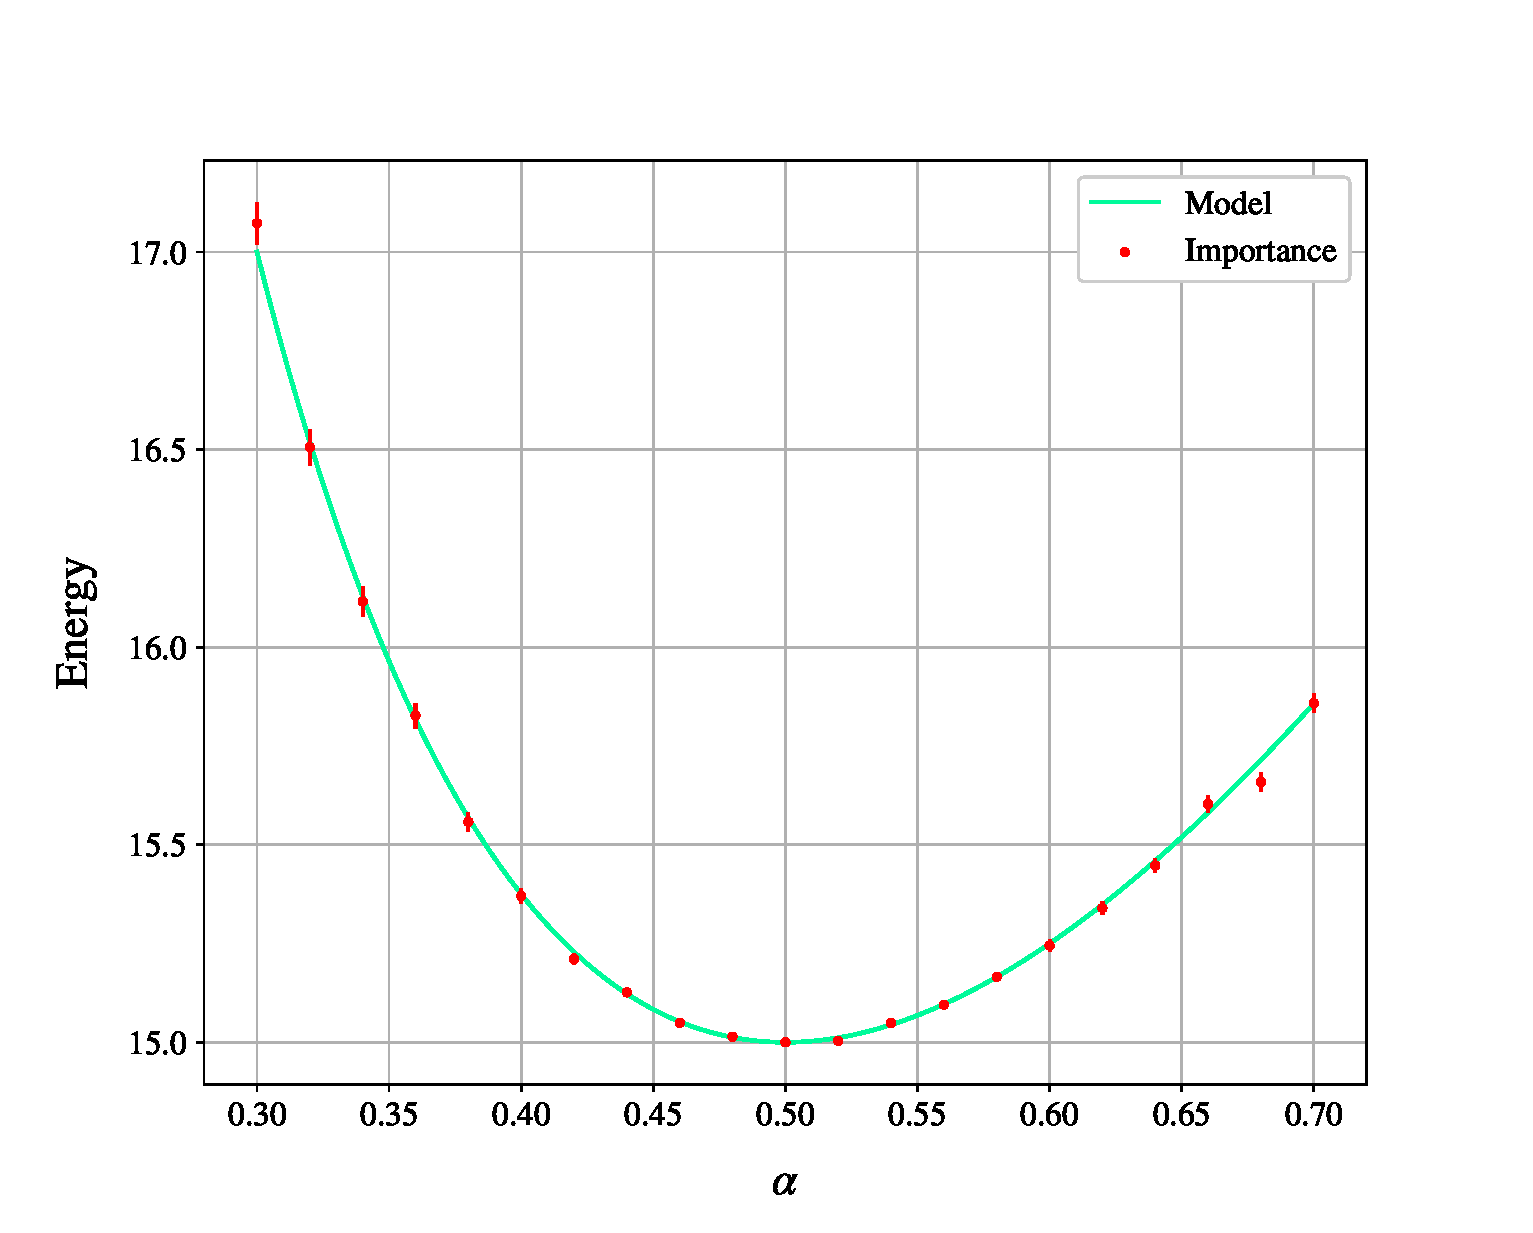
\includegraphics[scale=0.37]{images/varying_alpha_noninteract_importance.eps}
    \caption{The figure reports the energy estimates as a function of $\alpha$ generated by various VMC simulations exploiting the importance sampling with $N_{therm}=10^5$, $N_{steps}=2^{21}$, $\delta t = 0.1$. The curve is referred to a $3D$ system with $N=10$ non-interacting particles. For some of the points the errorbar is too small to be seen. }
    \label{fig:varying_alpha_noninteract_importance}
\end{figure}


\begin{table}[H]
    \centering
    \begin{tabular}{ccccc}
    \toprule
        \multicolumn{5}{c}{Metropolis} \\
        \midrule
        $\alpha$ & $\langle E_L \rangle$ & $\sigma_E$ & $\sigma_B$ & acc.ratio \\
         \midrule
        $0.3$ & 17.000 & 0.001 & 0.02 & 0.60313 \\
        $0.4$ & 15.3768 & 0.0006 & 0.007 & 0.54918 \\
        $0.5$ & 15.0000 & 0.0000 & 0.0000 & 0.50533 \\
        $0.6$ & 15.2492 & 0.0005 & 0.006 & 0.46724\\
        $0.7$ & 15.8461 & 0.0009 & 0.01 & 0.43341\\
        \midrule
        \midrule
         \multicolumn{5}{c}{Importance Sampling} \\
        \midrule
        $\alpha$ & $\langle E_L \rangle$ & $\sigma_E$ & $\sigma_B$ & acc.ratio \\
        \midrule
        $0.3$ & 16.9924 & 0.001 & 0.02 & 0.99343\\
        $0.4$ & 15.3826  & 0.0006 & 0.007 & 0.98982\\
        $0.5$ & 15.0000 & 0.0000 & 0.0000 & 0.98587 \\
        $0.6$ & 15.2471 & 0.0005 & 0.005 & 0.98123\\
        $0.7$ & 15.8468 & 0.0009 & 0.008 & 0.97630\\
        \bottomrule
    \end{tabular}
    \caption{Results of the simulations for different values of the variational parameter $\alpha$. Here $\sigma_E$ is the error on $\langle E_L \rangle$ estimated from the standard deviation of the $E_L$ samples generated during the run, while $\sigma_B$ comes from the blocking analysis. For both the brute-force Metropolis case and the importance sampling case we used 10 particles in 3 dimensions, $N_{therm}=10^5$ and $N_{steps}=2^{21}$. The chosen step-size for the Metropolis algorithm was $r_{step}=1.0$ and the time step-size for the Importance Sampling was $\delta t = 0.1$. }
    \label{tab:varying_alpha_noninteracting}
\end{table}

Even if simple and primitive, this model allowed us to test many of the fundamental parts of the code and made us understand how to fine-tune some parameters involved in the problem. For example, we analysed the effects of the time-step length $\delta t$ in the importance sampling case, concluding that a good choice for the parameter could be $\delta t = 0.1$. Our choice is justified by the fact that this value of $\delta t$ provides us both with a relatively high speed in the exploration of the space of configurations and a high acceptance ratio. In fact, it allows sufficiently large steps for the particles (according to Eq.\,\ref{new_position_importance}), still having number of accepted moves close to the actual number of performed steps. Both these aspects can be appreciated in Figure \ref{fig:dt_importance_sampling} and Figure \ref{fig:correlation_varying_dt}: the former shows the acceptance ratio as a function of $\delta t$, the latter demonstrates that a smaller value for the time-step introduces more correlation between data. For the realization of this second graph the parameter $\alpha$ was set to 0.4 in order to introduce some statistical fluctuations in the data, otherwise absent in the case of $\alpha=0.5$.


\begin{figure}[H]
    \centering
    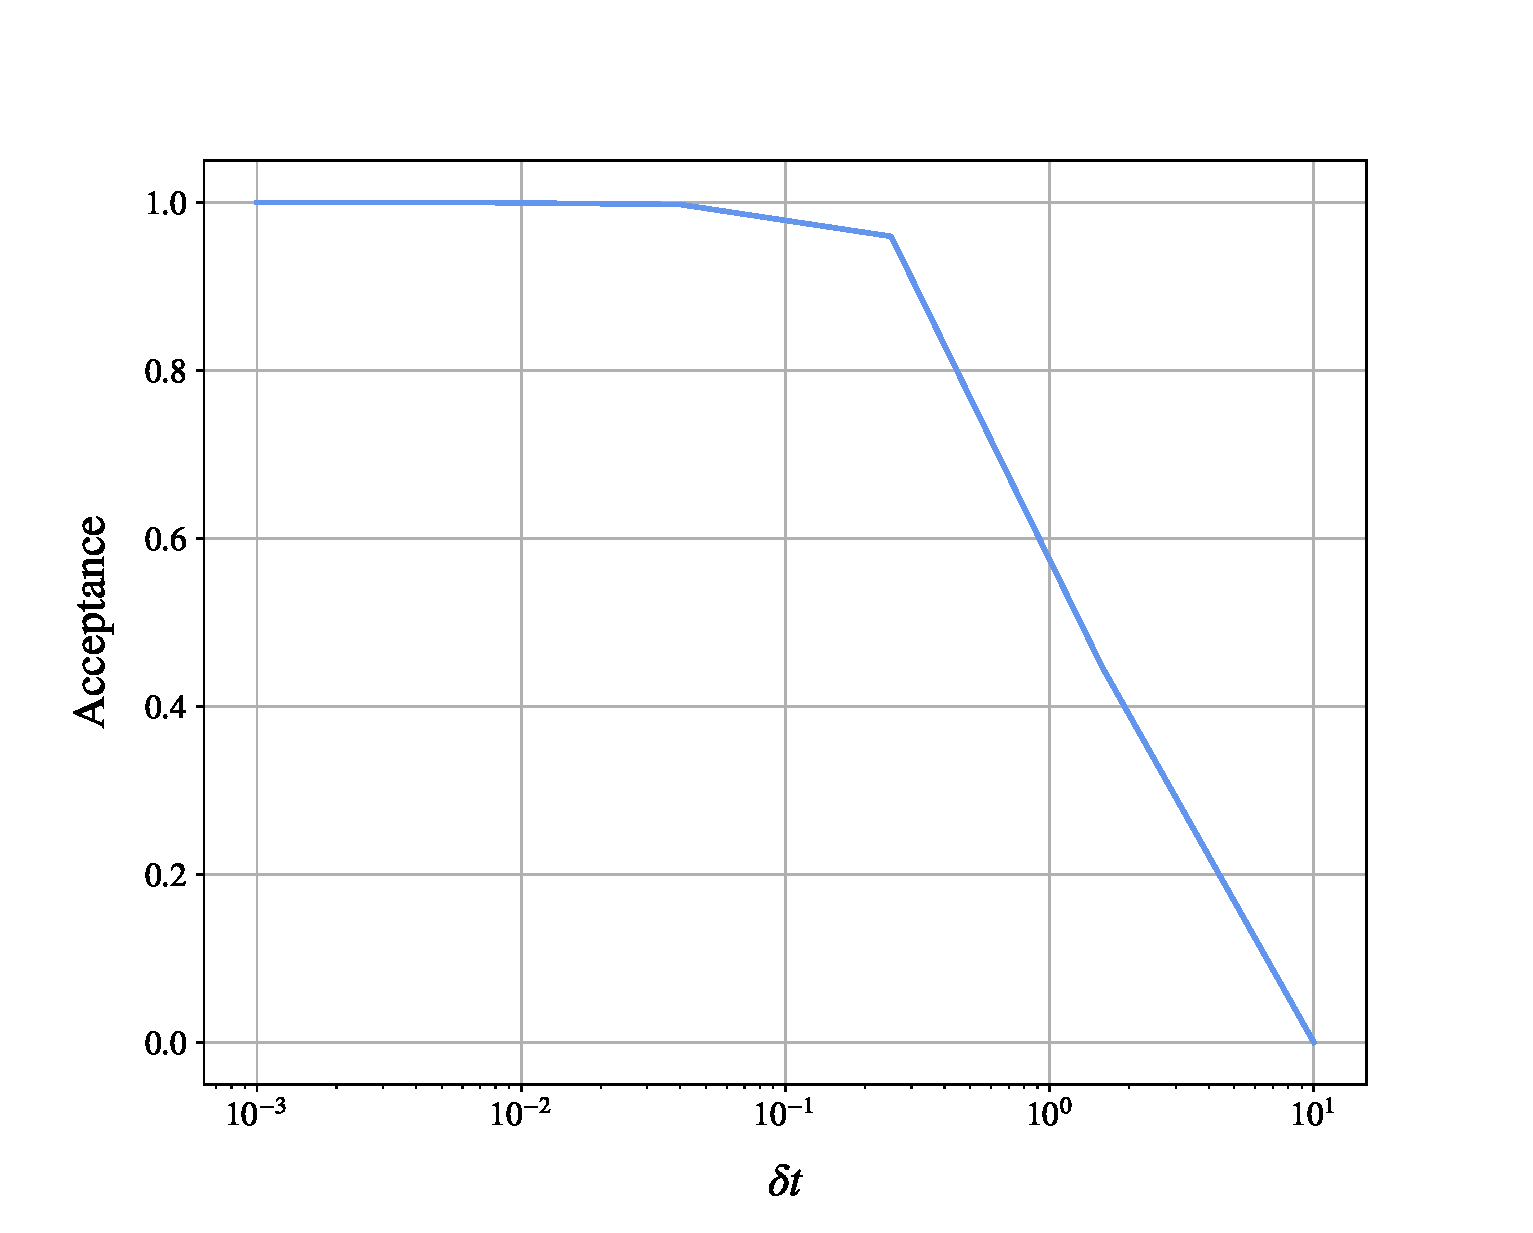
\includegraphics[scale=0.37]{images/varying_dt.eps}
    \caption{Acceptance ratio as a function of the time-step $\delta t$ in the context of VMC simulation performed with the importance sampling technique. Each run is conducted with $N_{therm}=10^5$, $N_{steps}=2^{21}$ and involves a system of $10$ non-interacting particles in 3-dimensions with $\alpha=0.5$.}
    \label{fig:dt_importance_sampling}
\end{figure}

\begin{figure}[H]
    \centering
    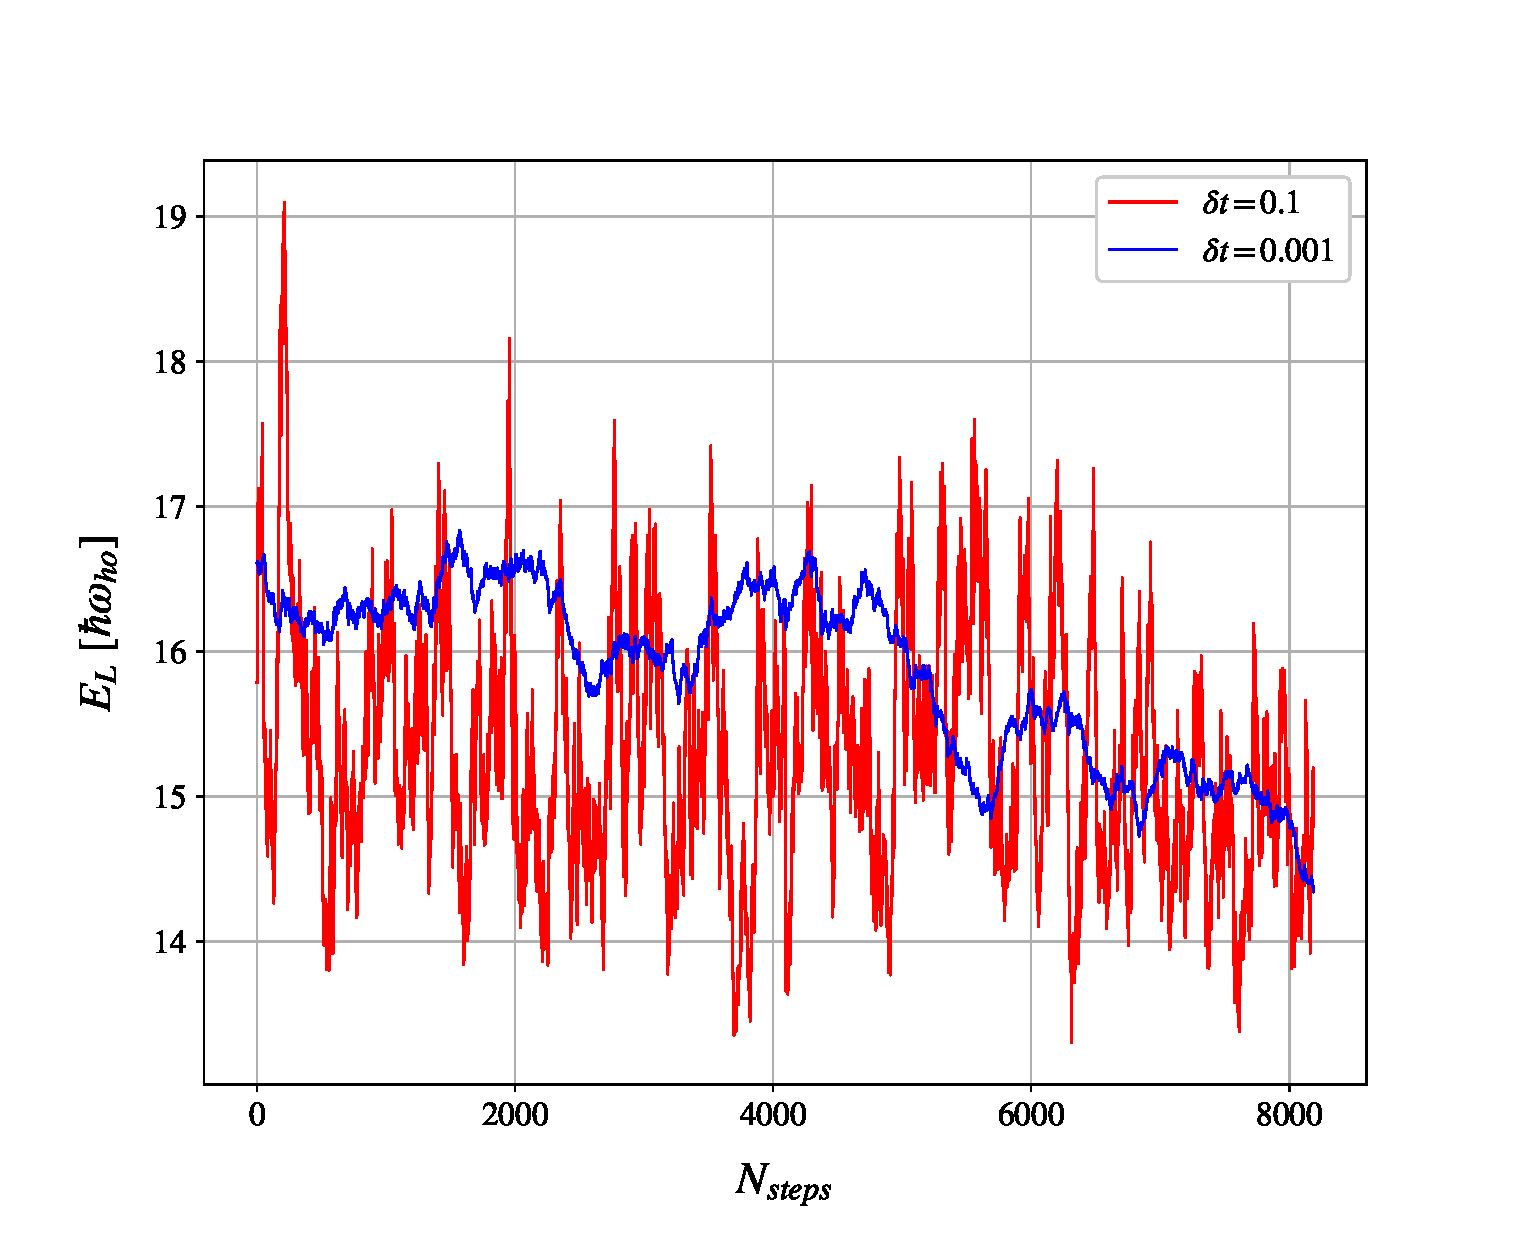
\includegraphics[scale=0.37]{images/correlation_different_deltat.eps}
    \caption{Local energy evaluated in each step of a VMC simulation after $N_{therm}=10^5$. A $3D$ system populated by 10 non-interacting particles inserted in a spherical potential is considered here. The image shows two curves for the chosen parameter $\delta t=0.001$ and $\delta t = 0.1$ used for the importance sampling method. The variational parameter $\alpha$ is set as constant to 0.4 to introduce some statistical fluctuations in the data, absent for $\alpha=0.5$. }
    \label{fig:correlation_varying_dt}
\end{figure}


\subsubsection{STATISTICAL ANALYSIS THROUGH BLOCKING METHOD}
As previously stated, Table \ref{tab:varying_alpha_noninteracting} contains estimations of the error affecting $\langle E_L(\alpha) \rangle$ obtained directly from the variance provided by the VMC simulations and the one obtained with the blocking technique. The python script that provided us with these latter results is based on the theoretical background described in Section \ref{sec:blocking_method}. The consistency of the mentioned script was also tested, in particular for what concerns the convergence of the estimate for  $\sigma_\mu^2$ (see Eq.\,\ref{eq:blocking_method}) to a finite value after a sufficiently high number of blocking iterations. In Figure \ref{fig:blocking_analysis} we present the values of $\sigma_k$ after each iteration of the mentioned method: the results are derived from a simulation performed with $2^{23}$ steps on a $3D$ system containing $N=10$ non-interacting particles inserted in a spherical potential. The sampling was performed through the Metropolis-Hastings algorithm using $\delta t=0.1$ and the variational parameter was again set to $\alpha=0.4$. As expected, we can observe that $\sigma_k$ reaches a plateau for sufficiently high values of $k$, and then an erratic behaviour enters into play, this due to the progressive reduction of the amount of points on which the variance is estimated. 

\begin{figure}[H]
    \centering
    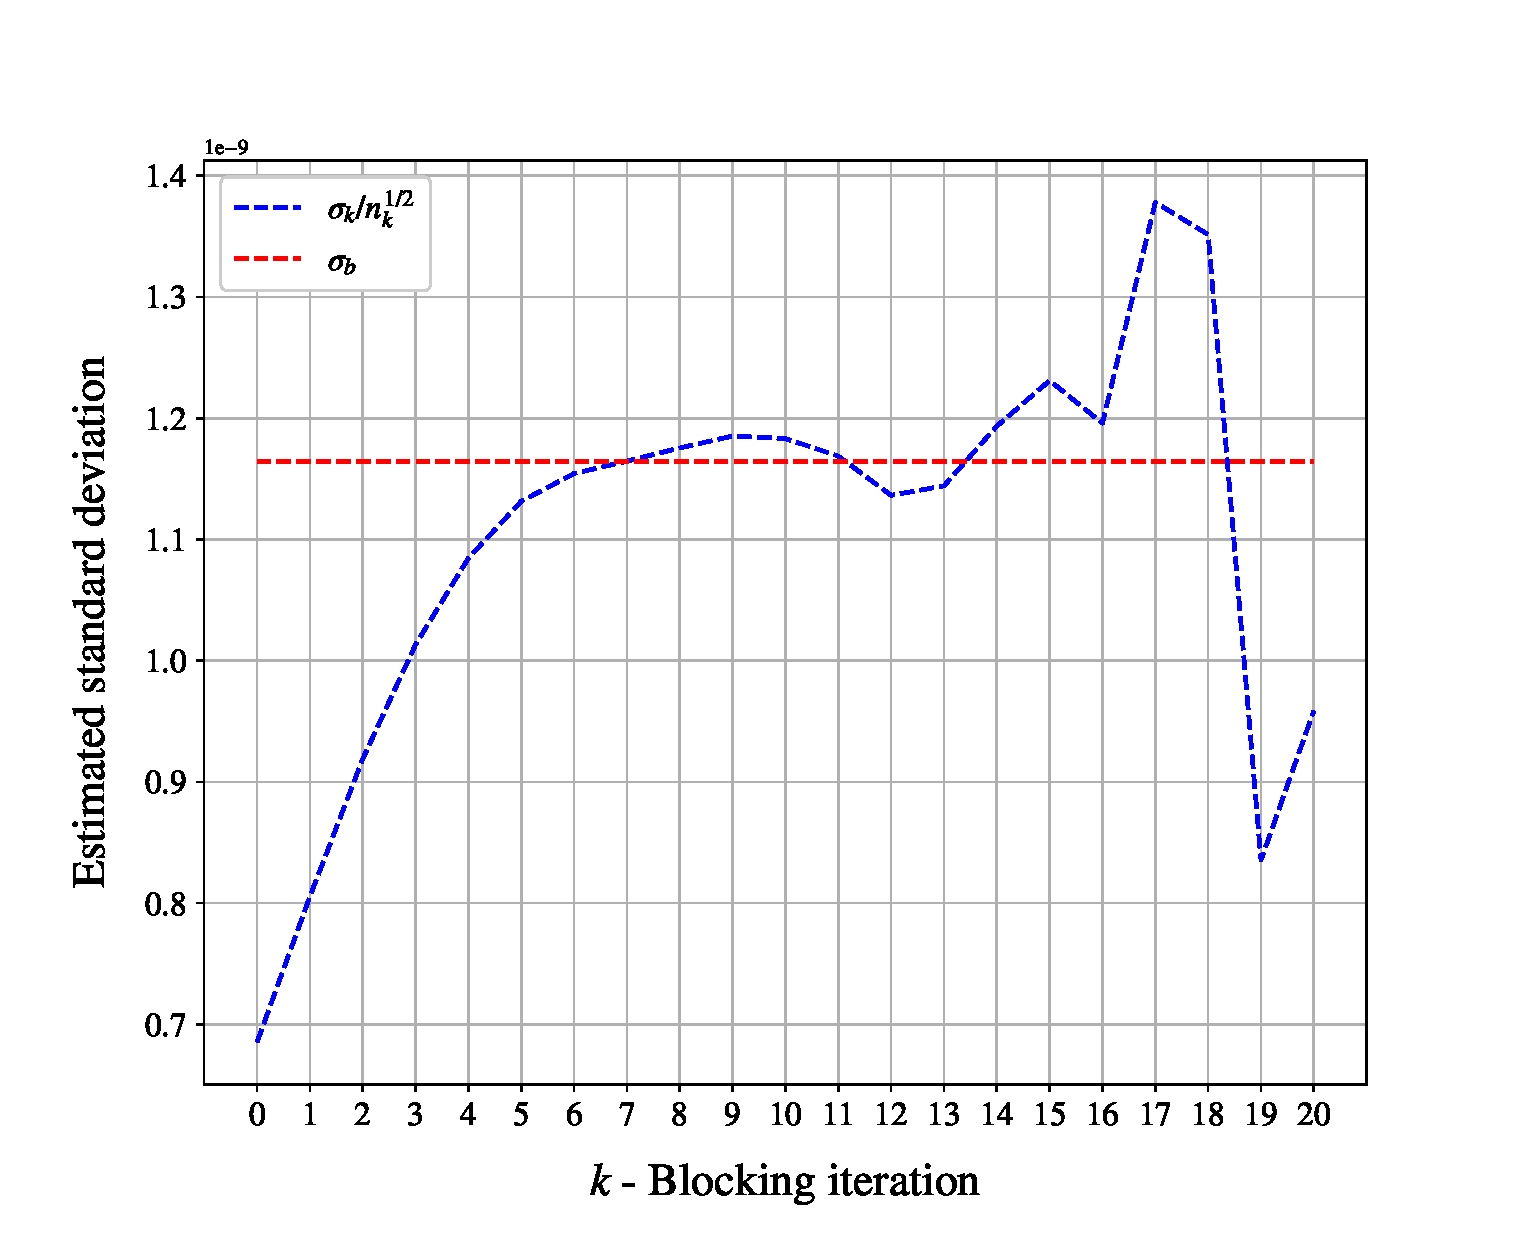
\includegraphics[scale=0.37]{images/sigma_blocking_behaviour.eps}
    \caption{The figure shows the behaviour of the variance estimate provided by the blocking technique implemented in a python script. The simulation was performed with $N_{therm}=10^5$ and $N_{steps}=2^{23}$ on a non-interacting $3D$ system characterized by $\alpha=0.4$ and populated by 10 particles. The Metropolis-Hastings algorithm with $\delta t =0.1$ was adopted for the sampling. }
    \label{fig:blocking_analysis}
\end{figure}


\subsection{INTERACTING CASE}
Subsequently we moved on to the interacting and asymmetrical case with trial wavefunction given by Eq.\,\ref{wavefunctions} and Hamiltonian described in Eq.\,\ref{hamiltonian} and Eq.\,\ref{elliptical_pot}. At first we compared results with those obtained from the symmetrical case, again to test the solidity of our code: this could be done by setting $\beta=1$, $w_z = w_{ho} = 1$ and the s-wave scattering length $a$ to 0. We verified that the results were coincident with those obtained in the non-interacting case, using both the Brute-force Metropolis algorithm and the importance sampling (see Appendix \ref{appendix:interacting_reduced_as_non_interacting}). From now on we will omit to specify the sampling algorithm used for each simulation, since all the next results were derived exploiting the Metripolis-Hastings one: this choice was driven by the fact that the this technique provides the combination of a higher acceptance ratio and better statistical sampling of the data. Furthermore, the variance on the energy value provided by each VMC was estimated through the blocking analysis. From now on, this information will be omitted too. \\

After the aforementioned consistency check we set the parameters' values $\omega_z = \beta = 2.82843$ and $a = 0.0043$ and ran the simulations for $N=10,50,100$ particles while varying $\alpha$. The simulations for 10 and 50 particles were carried out using $2^{21}$ steps, while in the case of 100 particles the high computational time imposed us a reduction of the number of steps to $2^{19}$. The parameter $\delta t = 0.1$ was the same for every run and the corresponding results are reported in Table \ref{tab:varying_alpha_noninteracting}. Furthermore, as an example the results obtained for 10 particles are reported in Figure \ref{fig:asymm_symm_comparison}, compared with their homologous obtained in the non-interacting symmetrical case. Figure \ref{fig:E_over_N} reports a comparison between the energy per particle as a function of the variational parameter $\alpha$ obtained for the three different values of $N$. \\



\begin{table}[H]
    \centering
    \begin{tabular}{cccc}
    \toprule
        \multicolumn{4}{c}{$N=10$} \\
        \midrule
        $\alpha$ & $\langle E_L \rangle$ & $\sigma_B$ & acc.ratio \\
        \midrule
        $0.3$ & 27.59 & 0.02 & 0.98185 \\
        $0.4$ & 24.969 & 0.008 & 0.97230 \\
        $0.5$ & 24.3991 & 0.0003 & 0.96178  \\
        $0.6$ & 24.822 & 0.006 & 0.94964 \\
        $0.7$ & 25.83 & 0.01 & 0.93758 \\
        \midrule
        \midrule
        \multicolumn{4}{c}{$N=50$} \\
        \midrule
        $\alpha$ & $\langle E_L \rangle$ & $\sigma_B$ & acc. ratio \\
        \midrule
        $0.3$ & 142.8 & 0.1 & 0.97840 \\
        $0.4$ & 129.81 & 0.04 & 0.96866 \\
        $0.5$ & 127.287 & 0.006 & 0.95759 \\
        $0.6$ & 129.90 & 0.03 & 0.94583 \\
        $0.7$ & 135.54 & 0.06 & 0.93361 \\
        \midrule
        \midrule
        \multicolumn{4}{c}{$N=100$} \\
        \midrule
        $\alpha$ & $\langle E_L \rangle$ & $\sigma_B$ & acc. ratio \\
        \midrule
        $0.3$ & 296.8 & 0.4 & 0.97610 \\
        $0.4$ & 271.2 & 0.1 & 0.96336 \\
        $0.5$ & 266.51 & 0.07 &  0.93323\\
        $0.6$ & 272.8 & 0.2 &   0.94392\\
        $0.7$ & 285.1 & 0.2 &  0.92906\\
        \bottomrule
    \end{tabular}
    \caption{The table reports the results of the simulations for different values of the variational parameter $\alpha$ for a $3D$ system constituted by $N=10,\;50,\;100$ particles. The simulations were performed exploiting the Metropolis-Hastings algorithm with $\delta t=0.1$, $N_{therm}=10^5$ and $N_{steps}=2^{21}$ for $N=10,\;50$, while and $N_{steps}=2^{19}$ for $N=100$. }
    \label{tab:varying_alpha_interacting}
\end{table}


\begin{figure}[H]
    \includegraphics[scale=0.37]{images/varying_alpha_comparison_interacting_and_not.eps}
    \caption{The figure reports the energy estimates as a function of $\alpha$ generated by various VMC simulations exploiting the importance sampling algorithm with $N_{therm}=10^5$, $N_{steps}=2^{21}$, $\delta t = 0.1$. The curves are referred to a $3D$ system populated respectively by 10 non-interacting particles in a spherical potential and 10 interacting particles in an elliptical potential. The errorbars are too small to be seen. }
    \label{fig:asymm_symm_comparison}
\end{figure}


\begin{figure}[H]
    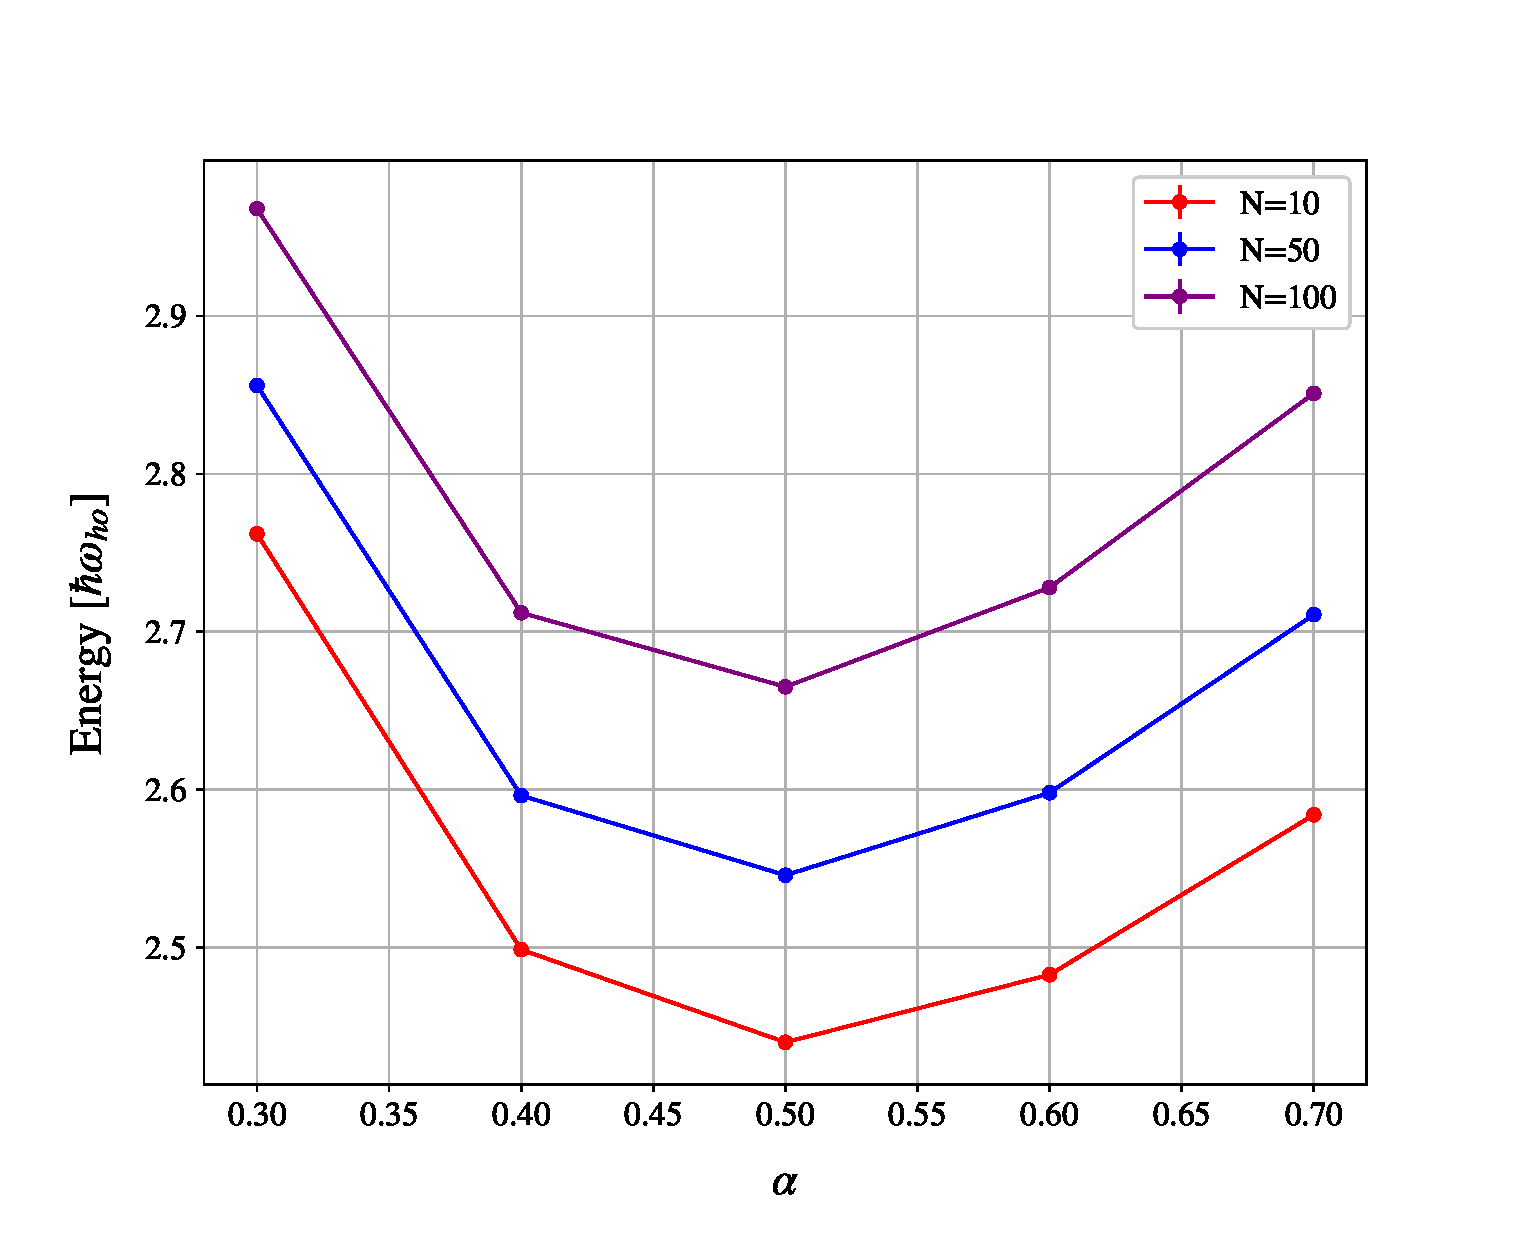
\includegraphics[scale=0.37]{images/energy_over_N.eps}
    \caption{The figure reports the average energy per particle as a function of $\alpha$ generated by various VMC simulations exploiting the importance sampling algorithm with $N_{therm}=10^5$ and $\delta t = 0.1$. The curves are referred to a $3D$ system populated respectively by 10, 50 and 100 interacting particles in an elliptical potential. The number of employed steps was $2^{21}$ for $N=10$ and $N=50$, while $2^{19}$ for $N=100$. }
    \label{fig:E_over_N}
\end{figure}


\subsection{GRADIENT DESCENT}
\label{sec:gradient_descent_results}
When considering the interaction between particles, the proof of the convexity of the function describing $\langle E_L \rangle$ as a function of $\alpha$ is non-trivial, thus in principle we can not state with absolute confidence that the curve is convex. However, as we can see from the latest figures, the behaviour of $\langle E_L \rangle$ as a function of $\alpha$ still encourages us to exploit the gradient descent method to research for  $\alpha_{GS}$ which minimizes the energy of the system. Before proceeding with the actual investigation in the interacting case, we tested the correct functioning of our code by applying it to a non-interacting system. In this simple case, it is well known that the optimal value of the variational parameter is $\alpha_{GS}=0.5$ and this result is independent of the number of particles and dimensionality. Therefore we expect to reach a convergence to this value whatever the adopted configuration. In particular, when considering particles without interaction we have at our disposal the analytical expression for the total energy of the system (see Eq.\,\ref{energy_analitical}) and the convexity of it is easy to prove. This ensures us that, if the method is capable in reaching a convergence for a sufficiently small value of the so-called learning rate $\gamma$ appearing in Eq.\,\ref{alpha_k}, the gradient descent will lead to a proper estimation of $\alpha_{GS}$. Table \ref{tab:gradient_descent_noninteracting} reports the results obtained with the application of the gradient descent method to a 3-dimensional system of 1, 10 and 100 non-interacting particles. Each VMC run was performed with $\delta t=0.1$ and $10^5$ thermalization steps, followed by another $10^5$ for the actual evaluation of the quantities reported in Eq.\,\ref{dEnergy_dalpha}. The learning rate was properly chosen for each configuration and the tolerance on the derivative was fixed to $\varepsilon=10^{-8}$ with no limit on the maximum number of iterations. The stability of the algorithm was also tested by performing the descent starting from two different guesses for the variational parameter, namely $\alpha_0=0.4$ and $\alpha_0=0.6$.


\begin{table}[H]
    \centering
    \begin{tabular}{ccccc}
    \toprule
        $N$ & $\gamma$ & $\alpha_0$ & $\alpha_{best}$ & $N_{conv}$ \\
        \midrule
        1 & 1\e-2 & 0.4 & 0.500 & 285 \\
        1 & 1\e-2 & 0.6 & 0.500 & 295 \\
        10 & 1\e-2 & 0.4 & 0.500 & 21 \\
        10 & 1\e-2 & 0.6 & 0.500 & 23 \\
        100 & 1\e-3 & 0.4 & 0.500 & 24 \\
        100 & 1\e-3 & 0.6 & 0.500 & 26 \\
        \bottomrule
    \end{tabular}
    \caption{Convergence analysis for the energy minimization process performed on a $3D$ non-interacting system of 1, 10, 100 particles in a spherical potential. The simulations were performed with $10^5$ steps for both thermalization and actual run, adopting the importance sampling with $\delta t = 0.1$, adjustable $\gamma$ and tolerance $\varepsilon=10^{-8}$. $N_{conv}$ refers to the number of gradient descent steps to get to convergence and $\alpha_0$ is the initial guess selected for the variational parameter.}
    \label{tab:gradient_descent_noninteracting}
\end{table}


Switching now to consider the interaction between particles, in this case the problem was less trivial, since the optimal value of the variational parameter depends also on the chosen number of particles and on the starting value of $\alpha$. Moreover, contrarily to the previous case, the exact value of $\alpha_{GS}$ is unknown and thus our research must be even more rigorous. However, the major limitation to precision here is constituted by the evaluation of the derivative of $\langle E_L \rangle$ with respect to $\alpha$. In fact, running a simple gradient descent with 10 particles, $\alpha_0=0.4$ and $\gamma=10^{-3}$ we observed that after some steps the derivative started oscillating between positive and negative values, always similar in magnitude between each others. The stochastic evaluation of this derivative enters here: in fact, even increasing the number of steps for each simulation or reducing the learning rate, we did not observe a further reduction of the derivative. Its values were always oscillating around zero, without decreasing in magnitude. We therefore retained to implement the method as follows: in the parallelized version of the code, each tread hosted a full gradient descent and for each number of particles we performed a first descent by adopting $\gamma=10^{-3}$ for a rapid convergence to a proximity of the result we aim at. When the aforementioned derivative started showing its oscillatory behaviour, a smaller $\gamma$ was selected and combined with a higher number of steps for each VMC simulation, this with the aim of increasing the precision in the evaluation of the derivative. If with these two improvements the algorithm still provided us with the above described oscillatory behaviour, the descent was interrupted and the selected $\alpha_{GS}$ is the average between the last values provided by each of the cores. Again the single runs were performed for $N=10,\,50,\,100$ using $10^5$ VMC steps and $\delta t =0.1$. For each $N$ the research of the optimal variational parameter was performed starting from 2 initial guesses. Our analysis is resumed in Table \ref{tab:gradient_descent_interacting}.

Once that the values of $\alpha_{GS}$ has been achieved for any selected configuration, we proceeded with a final VMC run to estimate the ground state energy for each apparatus. The results reported in Table \ref{tab:final_GS_energy} are referred to simulations performed with $\delta t = 0.1$ and with a number Monte Carlo steps varying with the number of particles involved in the system (this choice was caused by the huge amount of time required for the simulations involving a highly populated system). We selected $2^{27}$ MC steps for $N=10$, $2^{25}$ MC steps for $N=50$ and $2^{23}$ MC steps for $N=100$. 


\begin{table}[H]
    \centering
    \begin{tabular}{cccccc}
        \toprule
        $N$ & $\alpha_{0}$ & $\alpha_{best}$ & $\gamma_{min}$ & $N_{steps-max}$ & $N_{conv}$ \\
        \midrule
        10 & 0.4 & 0.49751 & 1\e-3 & 1\e5 & 74 \\
        10 & 0.6 & 0.49751 & 1\e-3 & 1\e5 & 74 \\
        50 & 0.4 & 0.48881 & 1\e-5 & 2\e5 & 21 \\
        50 & 0.6 & 0.48939 & 1\e-5 & 2\e5 & 21 \\
        100 & 0.4 & 0.481 & 1\e-5 & 5\e5 & 16 \\
        100 & 0.6 & 0.483 & 1\e-5 & 5\e5 & 11 \\
        \bottomrule
    \end{tabular}
    \caption{Convergence analysis for the energy minimization process performed on a interacting system of 10, 50 and 100 particles in a elliptical potential. A detailed description of the algorithm implemented for reaching these results is described in Paragraph \ref{sec:gradient_descent_results}. Here $\gamma_{min}$ and $N_{steps-max}$ are the minimum learning rate and maximum number of VMC steps used to perform a single run, while $N_{conv}$ is the iteration number at which the algorithm was stopped. Each run was performed employing the importance sampling with $\delta t = 0.1$ and $N_{therm}=10^5$. }
    \label{tab:gradient_descent_interacting}
\end{table}


\begin{table}[H]
    \centering
    \begin{tabular}{ccccc}
    \toprule
            $N$ & $\alpha^{GS}$ & $E$ & $\sigma_B$ & acceptance \\
            \midrule
            10 & 0.49751 & 24.39843 & 0.00003 & 0.96234 \\
            50 & 0.4891 & 127.48 & 0.07 & 0.94926 \\
            100 & 0.482 & 266.38 & 0.04 & 0.95036 \\
            \midrule
        \end{tabular}
    \caption{Results obtained for the ground state energy of a system of interacting particles in an elliptical potential. The final estimates were derived through VMC runs using the importance sampling method with $\delta t = 0.1$ and $10^{5}$ thermalization steps. We selected $N_{steps}=2^{27}$, $N_{steps}=2^{25}$ and $N_{steps}=2^{23}$ respectively for the systems in each of the 3 configurations with 10, 50 and 100 particles. The simulations were carried out exploiting the optimal variational parameter found after the gradient descent minimization and reported in Table \ref{tab:gradient_descent_interacting}. }
    \label{tab:final_GS_energy}
\end{table}




\subsection{ONE-BODY DENSITY}
With the energy-minimizing variational parameter at our disposal, we proceeded with the last step of our analysis, that is the previously introduced evaluation of the one-body density. Figure \ref{fig:one_body_density_histogram} shows the results obtained with the procedure described in section \ref{sec:one_body_density} applied to a system populated by 10 particles. For the construction of the curves reported below, the trial wavefunction of Eq.\,\ref{wavefunctions} was considered both with and without the Jastrow factor, varying the value of the parameter $a$ to amplify the effects introduced by the interaction term. In Figure \ref{fig:spatial_distribution_x_z} we represent also the spatial distribution of the particles along the $x$ and $z$ directions, in order to show the effects introduced by the modifications of the trap shape. The curves are referred to a system populated respectively by 10, 50 and 100 particles. Each of the simulations performed for this section were carried out with $\delta t = 0.1$ and $2^{23}$ steps, setting the $\alpha$ value to those reported in Table \ref{tab:final_GS_energy}.


\begin{figure}[H]
    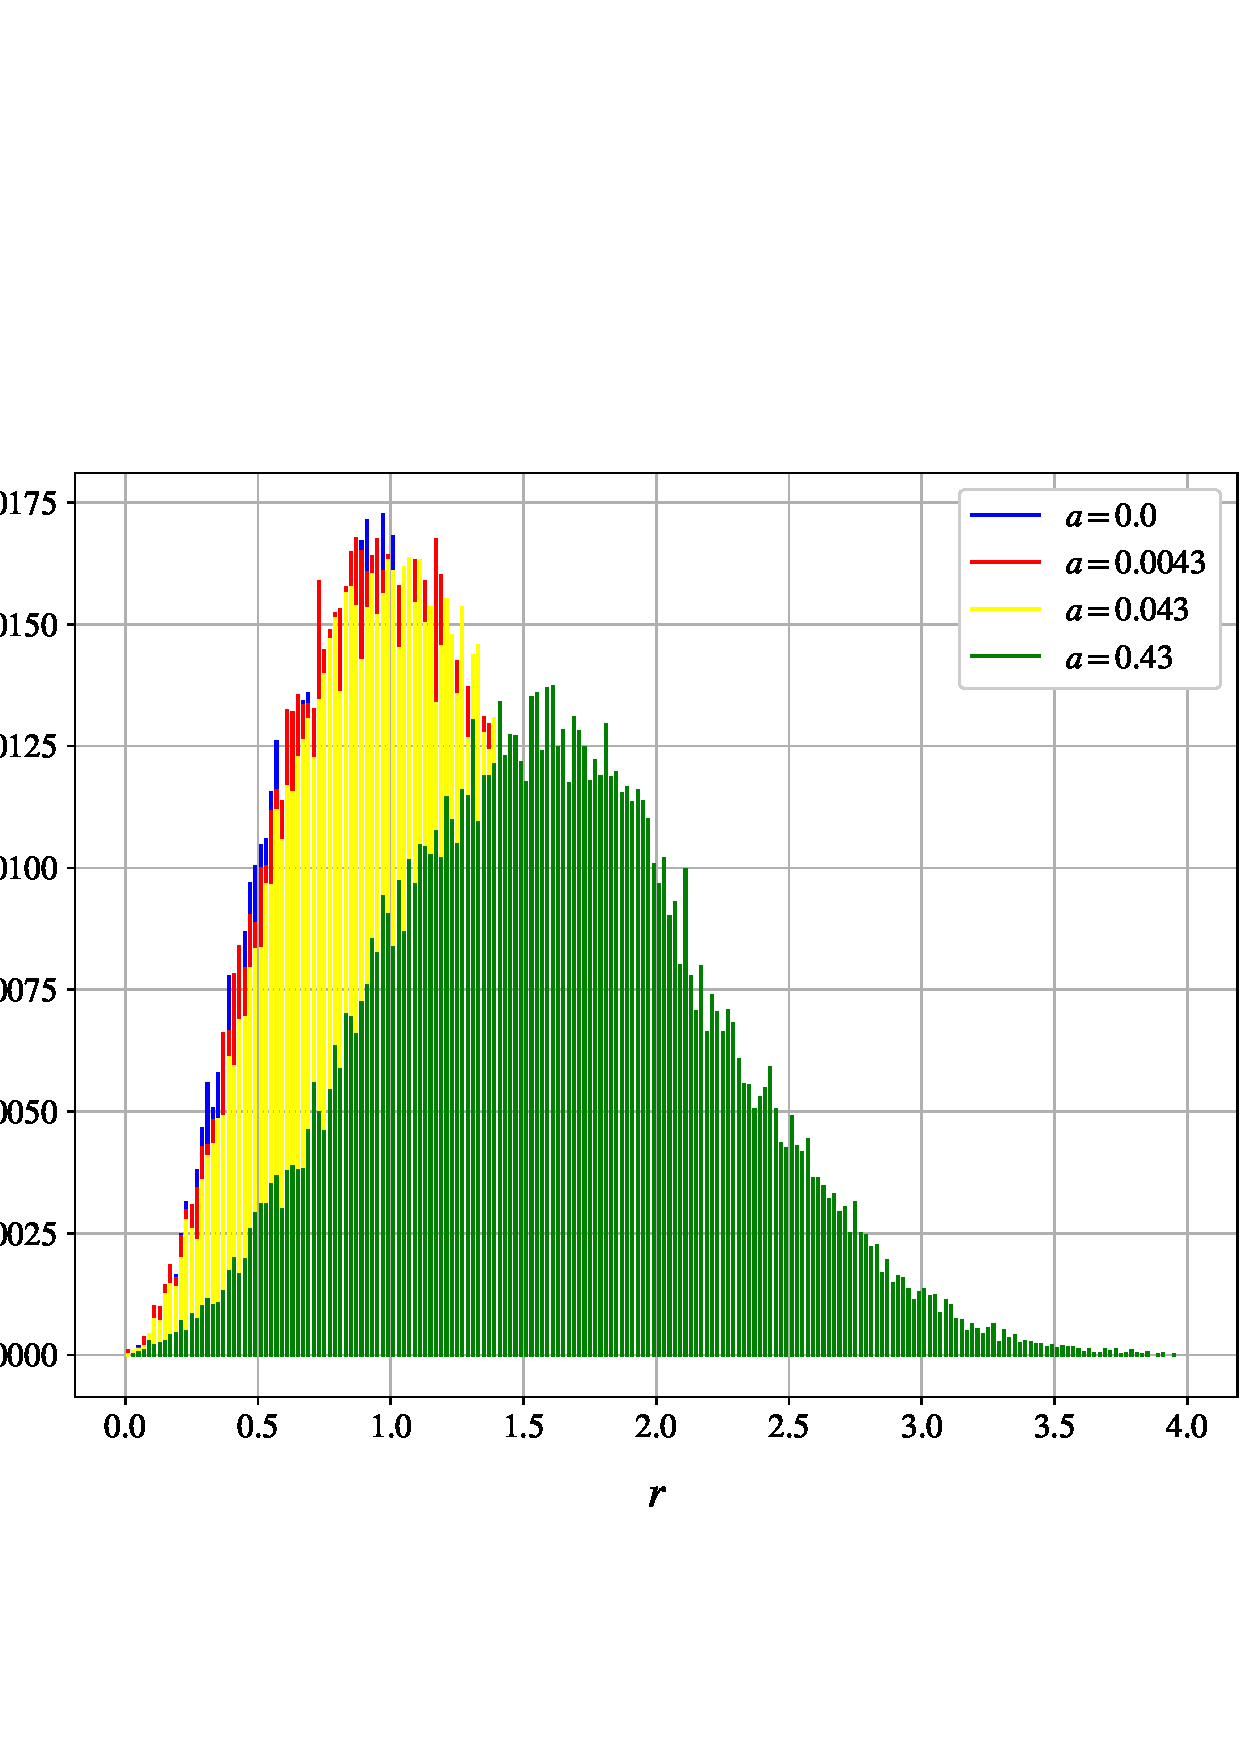
\includegraphics[scale=0.37]{images/onebody_density.jpg}
    \caption{One-body density as a function of the radial distance from the center of the chosen reference frame for a $3D$ system with $N=10$ particles described by an asymmetric gaussian wavefunction and inserted in a elliptical potential. The histograms are built for different values of $a$ in order to increase the effects introduced by the Jastrow factor in the wavefunction. The simulations were carried our exploiting the importance sampling with $N_{therm}=10^5$, $N_{steps}=2^{23}$, $\delta t =0.1$ and the $\alpha$ value deriving from the minimization of the energy (reported in Table \ref{tab:gradient_descent_interacting}). Notice that the curves for $a=0$ and $a=0.0043$ are almost perfectly overlapped. }
    \label{fig:one_body_density_histogram}
\end{figure}

\begin{figure}[H]
    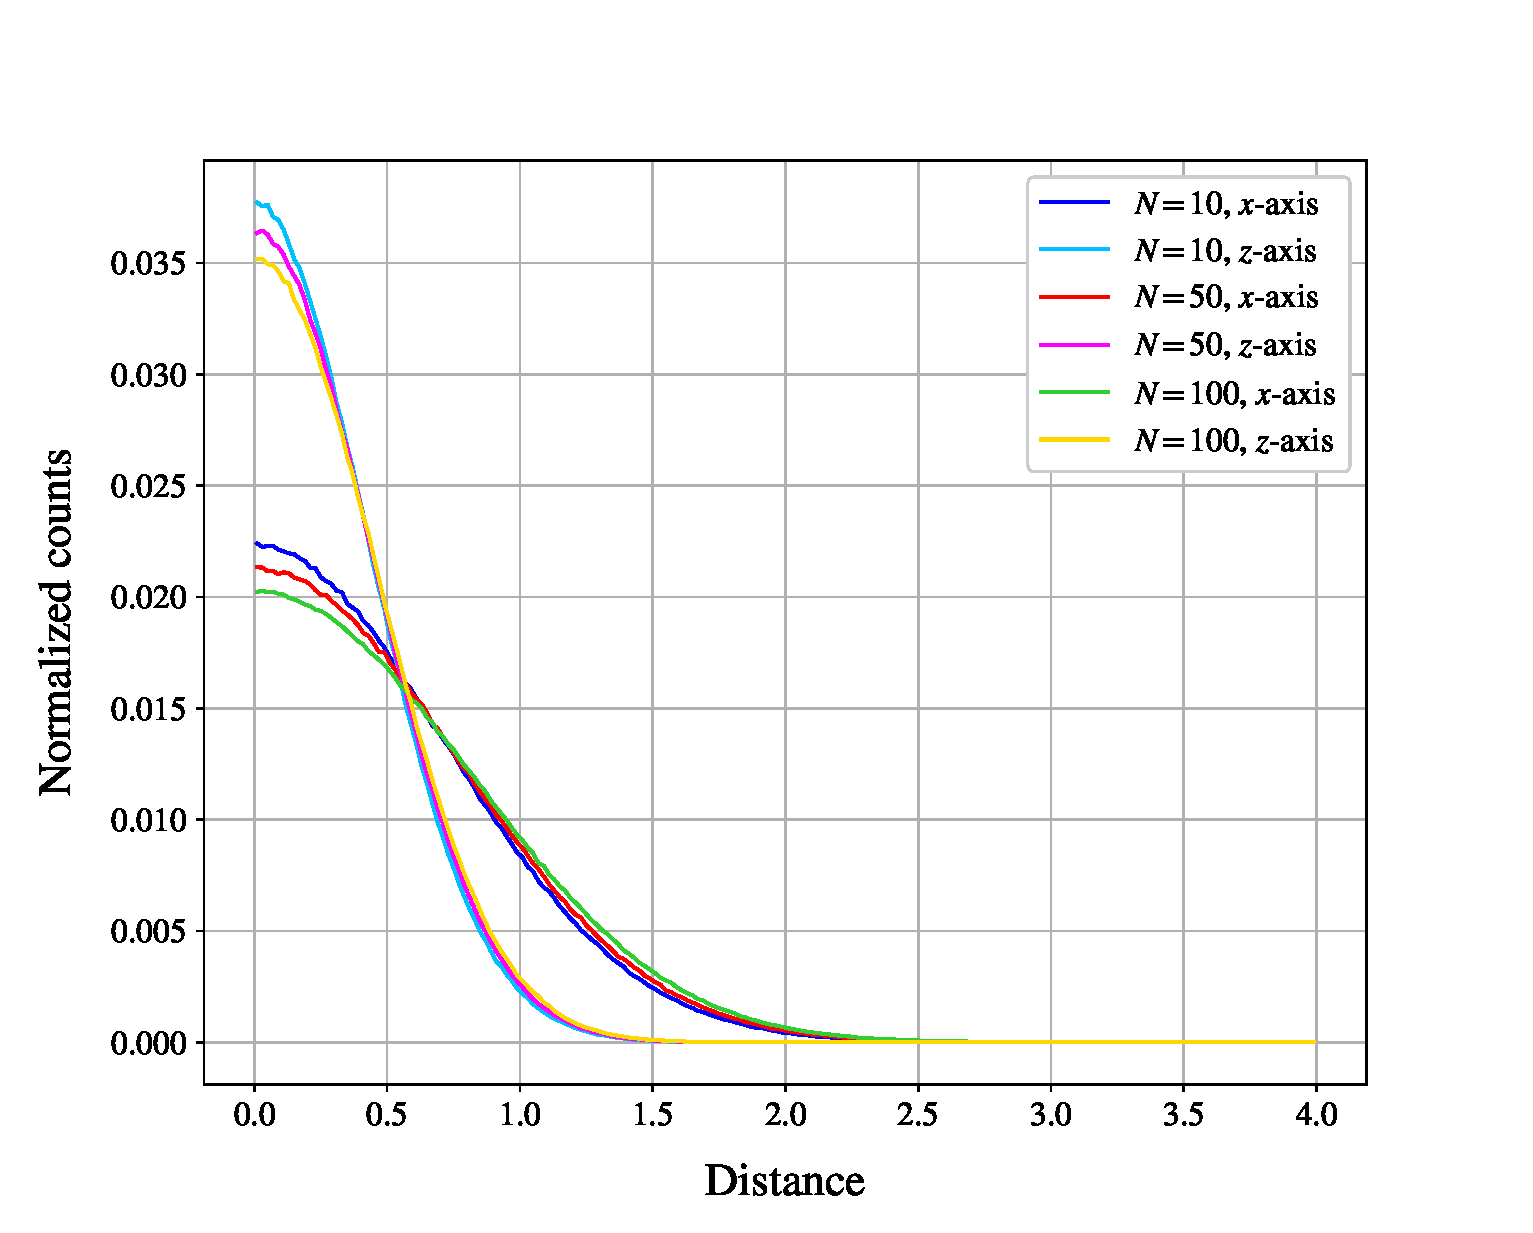
\includegraphics[scale=0.37]{images/spatial_distribution_x_z.eps}
    \caption{Particles' spatial distribution along the coordinates $x$ and $z$ for a system populated respectively by 10, 50 and 100 particles described by an asymmetric gaussian wavefunction and inserted in a elliptical potential. The simulations were carried our exploiting the importance sampling with $N{therm}=10^5$, $N_{steps}=2^{23}$ steps and $\delta t =0.1$, setting $\alpha$ to the values reported in Table \ref{tab:gradient_descent_interacting}. }
    \label{fig:spatial_distribution_x_z}
\end{figure}